\documentclass[aspectratio = 169]{beamer}
\usetheme{CambridgeUS}
\usecolortheme{beaver}
\usepackage{tikz}
\usepackage{graphicx}  
\usepackage{amsmath, amssymb}
\usepackage{hyperref}

\title{Michelson Experiment Summary}
\author{Yongao Hu}
\institute{MIT Department of Physics}
\date{\today}

\begin{document}

% \AtBeginSection[]
% {
%     \begin{frame}
%         \frametitle{Outline}
%         \tableofcontents[currentsection,currentsubsection]
%     \end{frame}
% }

% Title Slide
\begin{frame}
    \titlepage
\end{frame}

% Outline Slide
\begin{frame}{Outline}
    \tableofcontents
\end{frame}

% Introduction Slide
\section{The History of Michelson Interferometer}
\begin{frame}{The History of Michelson Interferometer}
    \begin{itemize}
        % \item Light exhibits interference when two waves overlap.
        \item The Michelson interferometer is designed by Albert Michelson.
        \item Historically, it disproved the existence of the "luminiferous aether" and contributed to the discovery of relativity.
        \item Interferometers are used in:
        \begin{itemize}
            \item Precision measurements
            \item LIGO for detecting gravitational waves \cite{LIGO2016}
        \end{itemize}
    \end{itemize}
\end{frame}

% Theory Slide
\section{Theoretical background: Interference of Light}
\begin{frame}{Interference of Light Waves}
    \begin{itemize}
        \item The interference pattern depends on the phase difference:
        \[
        \Delta \phi = 2\pi \frac{\Delta x}{\lambda}
        \]
        \item Intensity of interference:
        \[
        I = I_0 \cos^2(\Delta \phi)
        \]
        \item Maximum interference: $\Delta \phi = 2\pi n$
        \item Minimum interference: $\Delta \phi = (2n+1)\pi$
    \end{itemize}
\end{frame}

\begin{frame}{Interference of Light Waves}
\begin{columns}
    \column{0.5\textwidth}
    \begin{itemize}
        \item The interference pattern depends on the phase difference:
        \[
        \Delta \phi = 2\pi \frac{\Delta x}{\lambda}
        \]
        \item Intensity of interference:
        \[
        I = I_0 \cos^2(\Delta \phi)
        \]
        \item Maximum interference: $\Delta \phi = 2\pi n$
        \item Minimum interference: $\Delta \phi = (2n+1)\pi$
    \end{itemize}

    \column{0.5\textwidth}

    \begin{figure}
        \centering
        % ---------------------- Constructive Interference ----------------------
        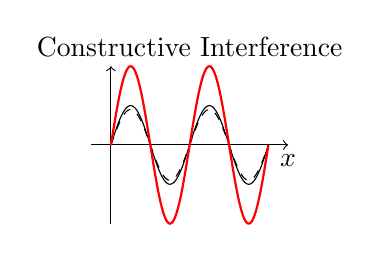
\begin{tikzpicture}[scale=0.5]
            % Axes
            \draw[->] (-0.5,0) -- (4.5,0) node[below]{$x$};
            % \draw[->] (0,-2) -- (0,2) node[left]{Amplitude};
            \draw[->] (0,-2) -- (0,2);

            % Wave 1
            \draw[samples=100,domain=0:4] 
                plot(\x,{sin(2*180*\x/2)}) 
                node[right] {};
            % Wave 2 (in phase with wave 1)
            \draw[dashed,samples=100,domain=0:4] 
                plot(\x,{0.9*sin(2*180*\x/2)}) 
                node[right] {};
            % Sum (constructive)
            \draw[thick,red,samples=100,domain=0:4] 
                plot(\x,{2*sin(2*180*\x/2)}) 
                node[right] {};
            
            \node at (2,2.5) {Constructive Interference};
        \end{tikzpicture}

        \vskip1em  % Vertical space between the two plots

        % ---------------------- Destructive Interference ----------------------
        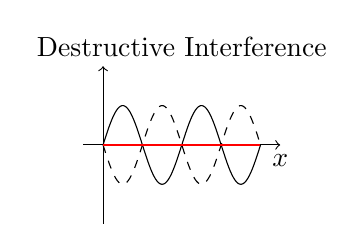
\begin{tikzpicture}[scale=0.5]
            % Axes
            \draw[->] (-0.5,0) -- (4.5,0) node[below]{$x$};
            % \draw[->] (0,-2) -- (0,2) node[left]{Amplitude};
            \draw[->] (0,-2) -- (0,2);

            % Wave 1
            \draw[samples=100,domain=0:4] 
                plot(\x,{sin(2*180*\x/2)}) 
                node[right] {};
            % Wave 2 (out of phase by pi)
            \draw[dashed,samples=100,domain=0:4] 
                plot(\x,{-sin(2*180*\x/2)}) 
                node[right] {};
            % Sum (destructive)
            \draw[thick,red,samples=100,domain=0:4] 
                plot(\x,{sin(2*180*\x/2) + (-sin(2*180*\x/2))}) 
                node[right] {};

            \node at (2,2.5) {Destructive Interference};
        \end{tikzpicture}

        \caption{Solid/dash lines: individual waves. Red lines: resultant waves}
    \end{figure}
\end{columns}
\end{frame}

\begin{frame}{Visibility of the Interference Pattern Measures how Resolved the Pattern is}
    \begin{itemize}
        \item Visibility measures how well the pattern is resolved:
        \[
        V = \frac{I_{\text{max}} - I_{\text{min}}}{I_{\text{max}} + I_{\text{min}}}
        \]
        \item Ideal case: $V = 1$
        \item Low visibility $\Rightarrow$ poor alignment or coherence issues
    \end{itemize}
\end{frame}

\begin{frame}{Piezoelectric Transducer Controls the Path Difference}
    \begin{itemize}
        \item A piezoelectric transducer moves a mirror in response to voltage.
        \item This changes the path length $\Delta x$ proportional to voltage.
        \item The wavelength of light is found using:
        \[
        \lambda = 4 \Delta V \times \frac{\Delta L}{V}
        \]
    \end{itemize}
\end{frame}

% Experimental Setup Slide
\section{Experimental Setup: the Interferometer}
\begin{frame}{Michelson Interferometer Setup}
  \begin{columns}
    % Left column
    \column{0.5\textwidth}
      \begin{itemize}
        \item Light source: laser
        \item 50/50 beam splitter splits the light into two paths.
        \item One mirror is stationary, the other mounted on a piezoelectric transducer.
        \item Detector: photodiode (voltage output proportional to intensity).
        \item Signal generator applies a triangular voltage to move the mirror.
      \end{itemize}

    % Right column
    \column{0.5\textwidth}
      \begin{figure}
          \centering
          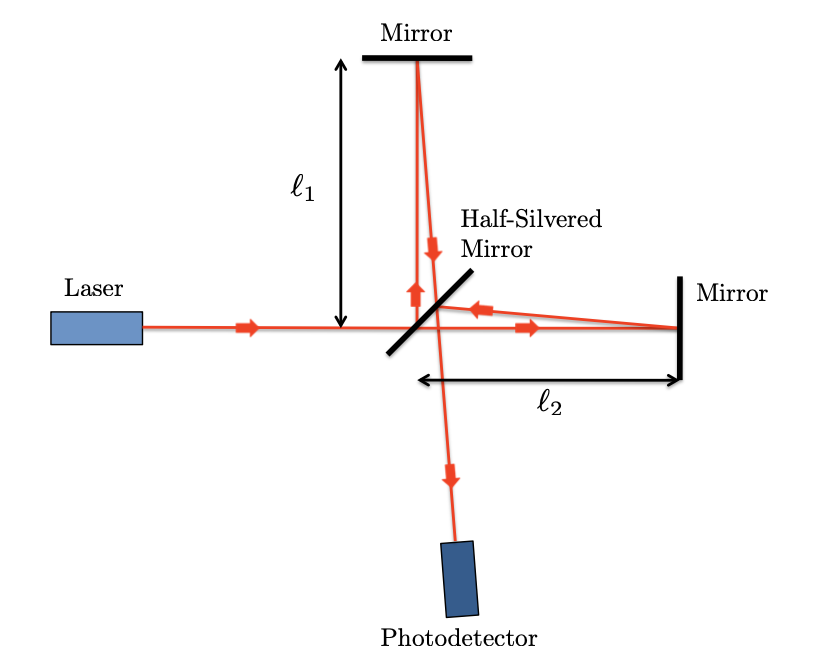
\includegraphics[width=0.8\textwidth]{fig/michelson_setup.png}
          \caption{Schematic of the Michelson interferometer. Adapted from \cite{MITOpticalInterferometry2023}.}
      \end{figure} 
  \end{columns}
\end{frame}

\section{Data Analysis: Detection of Minima and Maxima}
\begin{frame}{Data Processing and Interference Pattern Visibility}
\begin{columns}
    \column{0.5\textwidth}
    \begin{itemize}
        \item Voltage signals recorded from signal generator and photodiode.
        \item Used \texttt{findpeak} in \texttt{SciPy} to locate primary maxima and minima.
        \item Applied \texttt{KMeans} clustering (\texttt{SciKit-Learn}) to group voltage values.
        % \item Measured $\Delta V$ between consecutive maxima and minima.
    \end{itemize}
    
    \column{0.5\textwidth}
        \begin{figure}
        \centering
        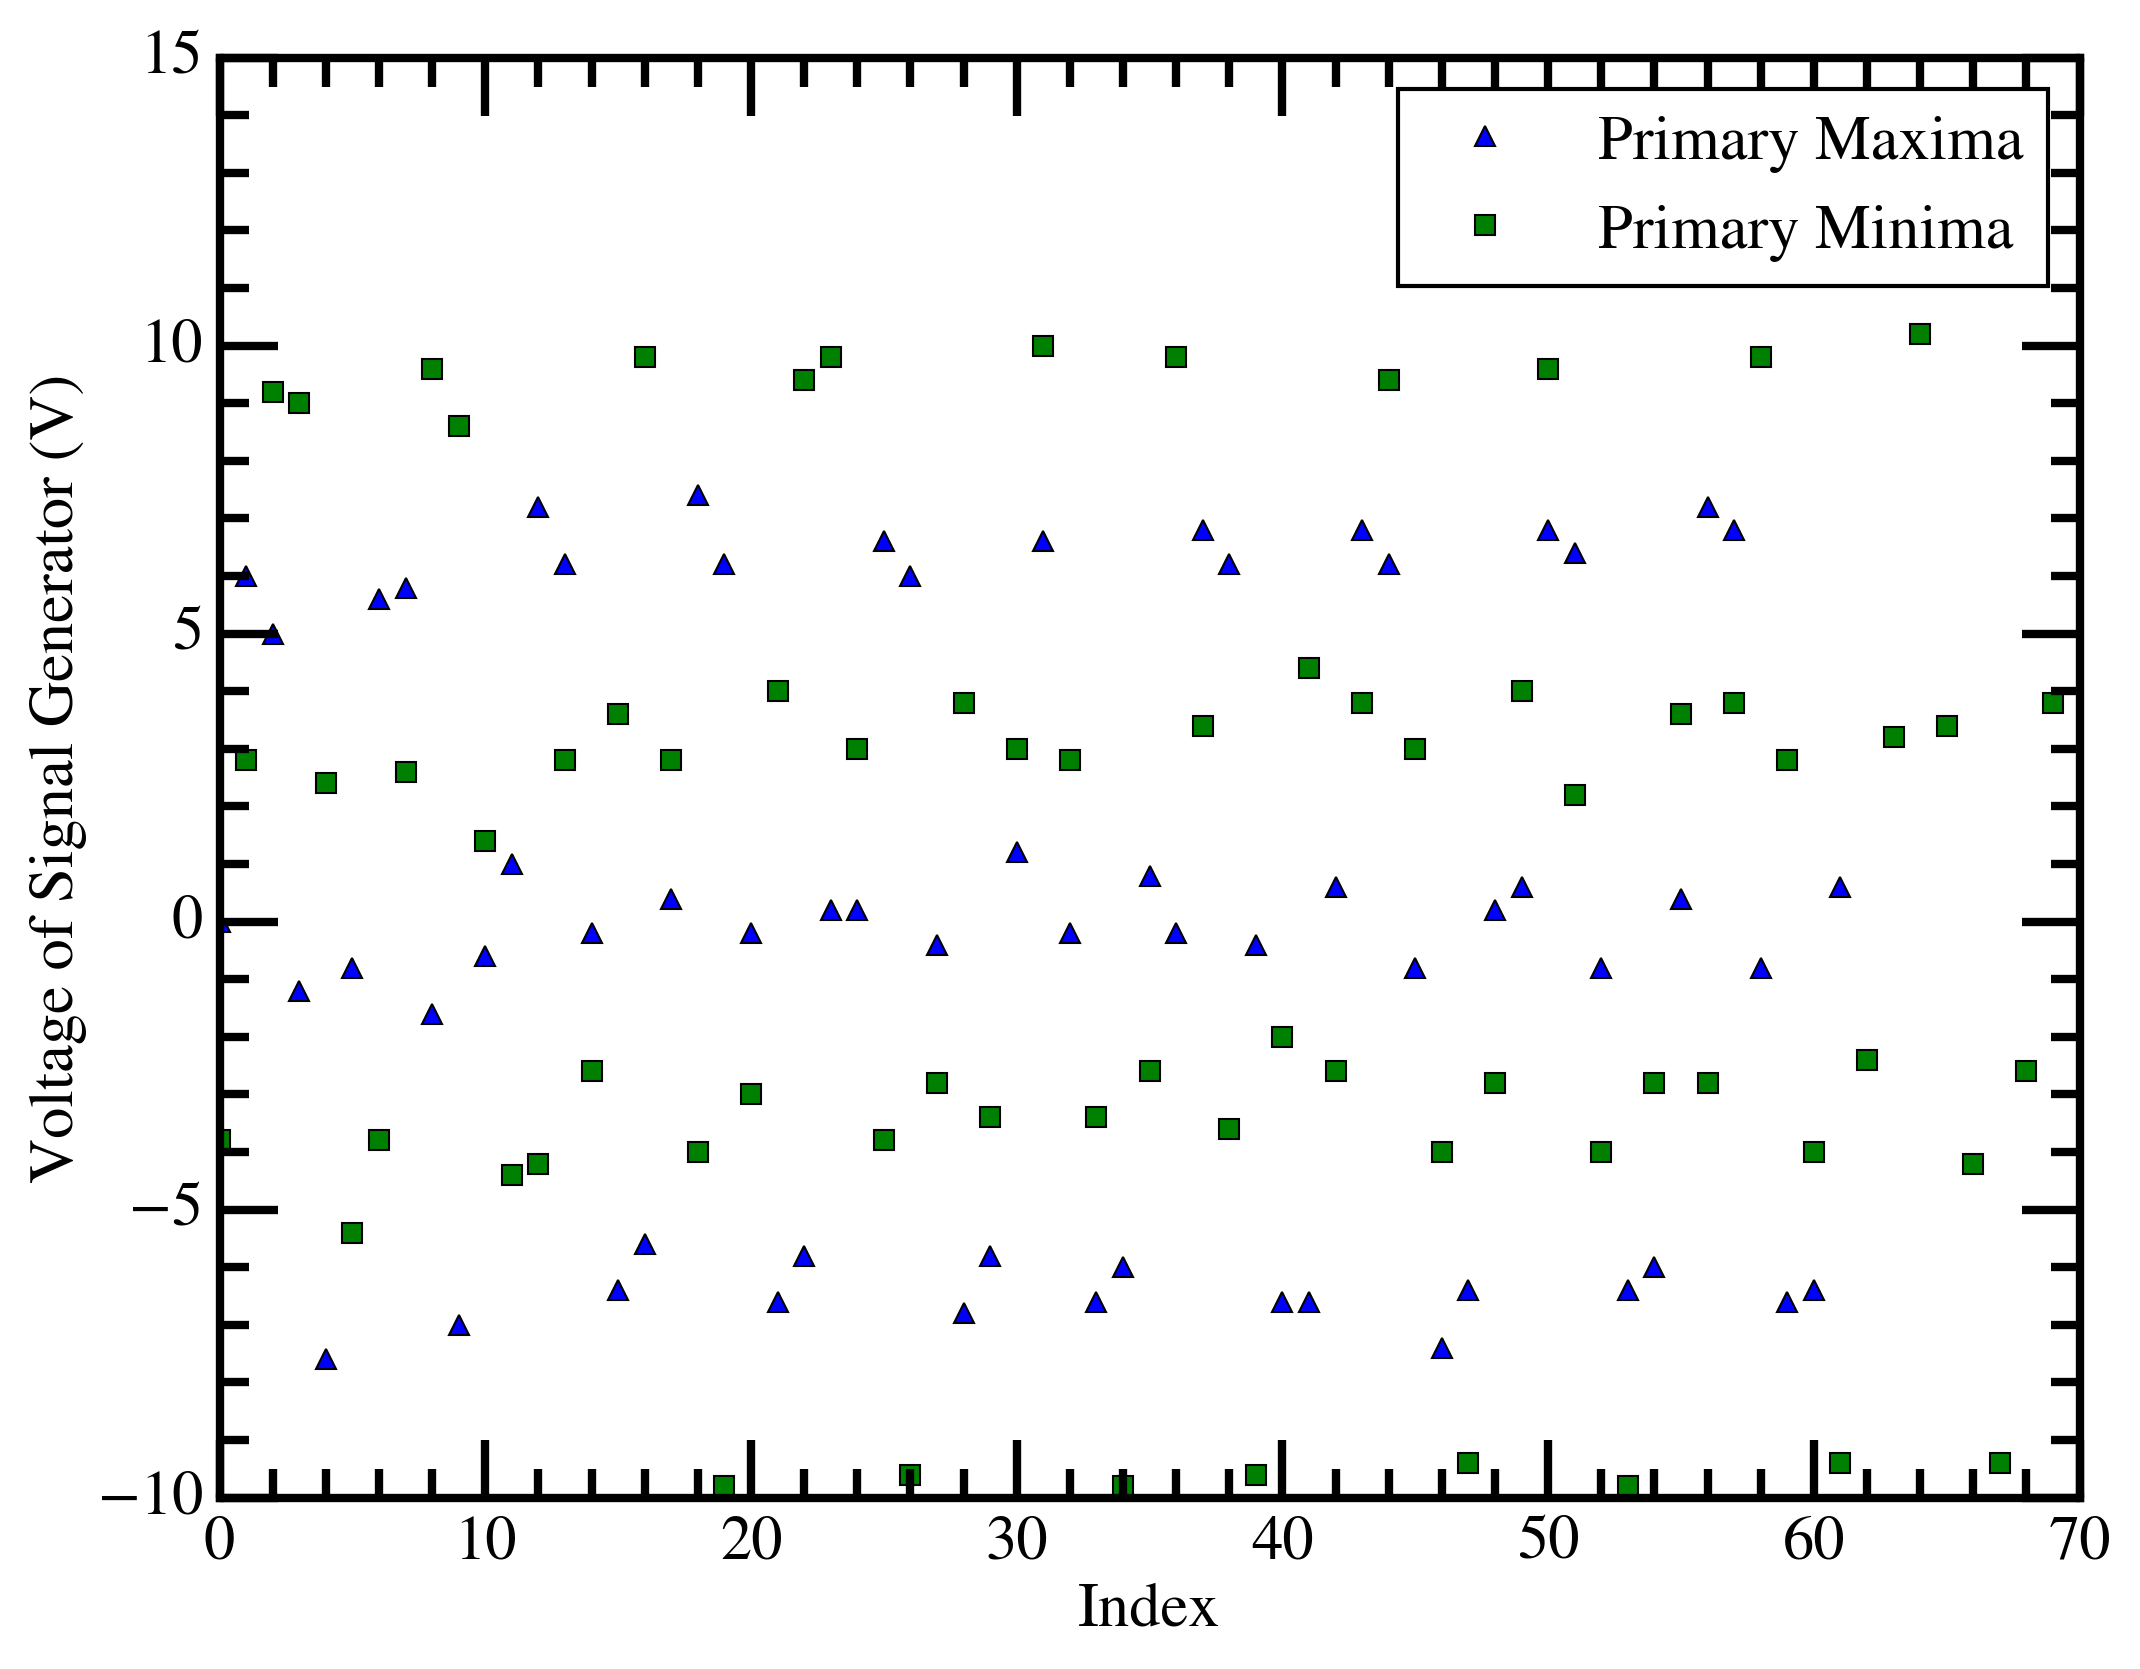
\includegraphics[width=0.8\textwidth]{fig/Primary_Maxima_Minima.png}
    \caption{Voltage at primary maxima and minima.}
    \end{figure}
\end{columns}

\end{frame}

% Results Slide
\section{Results: Visibility and Wavelength of the Laser}

\begin{frame}{Visibility $0.179\pm 0.001$ Not Perfect but Significant}
\begin{columns}
    \column{0.5\textwidth}
    \begin{itemize}
        \item Maximum voltage: $(1.592\pm0.002)\text{ V}$
        \item Minimum voltage: $(1.110\pm0.002)\text{ V}$
        \item Visibility:
        \[
        V = 0.179\pm0.001
        \]
        \item Imperfect alignment likely lowered visibility.
    \end{itemize}
    
    \column{0.5\textwidth}
        \begin{figure}
        \centering
        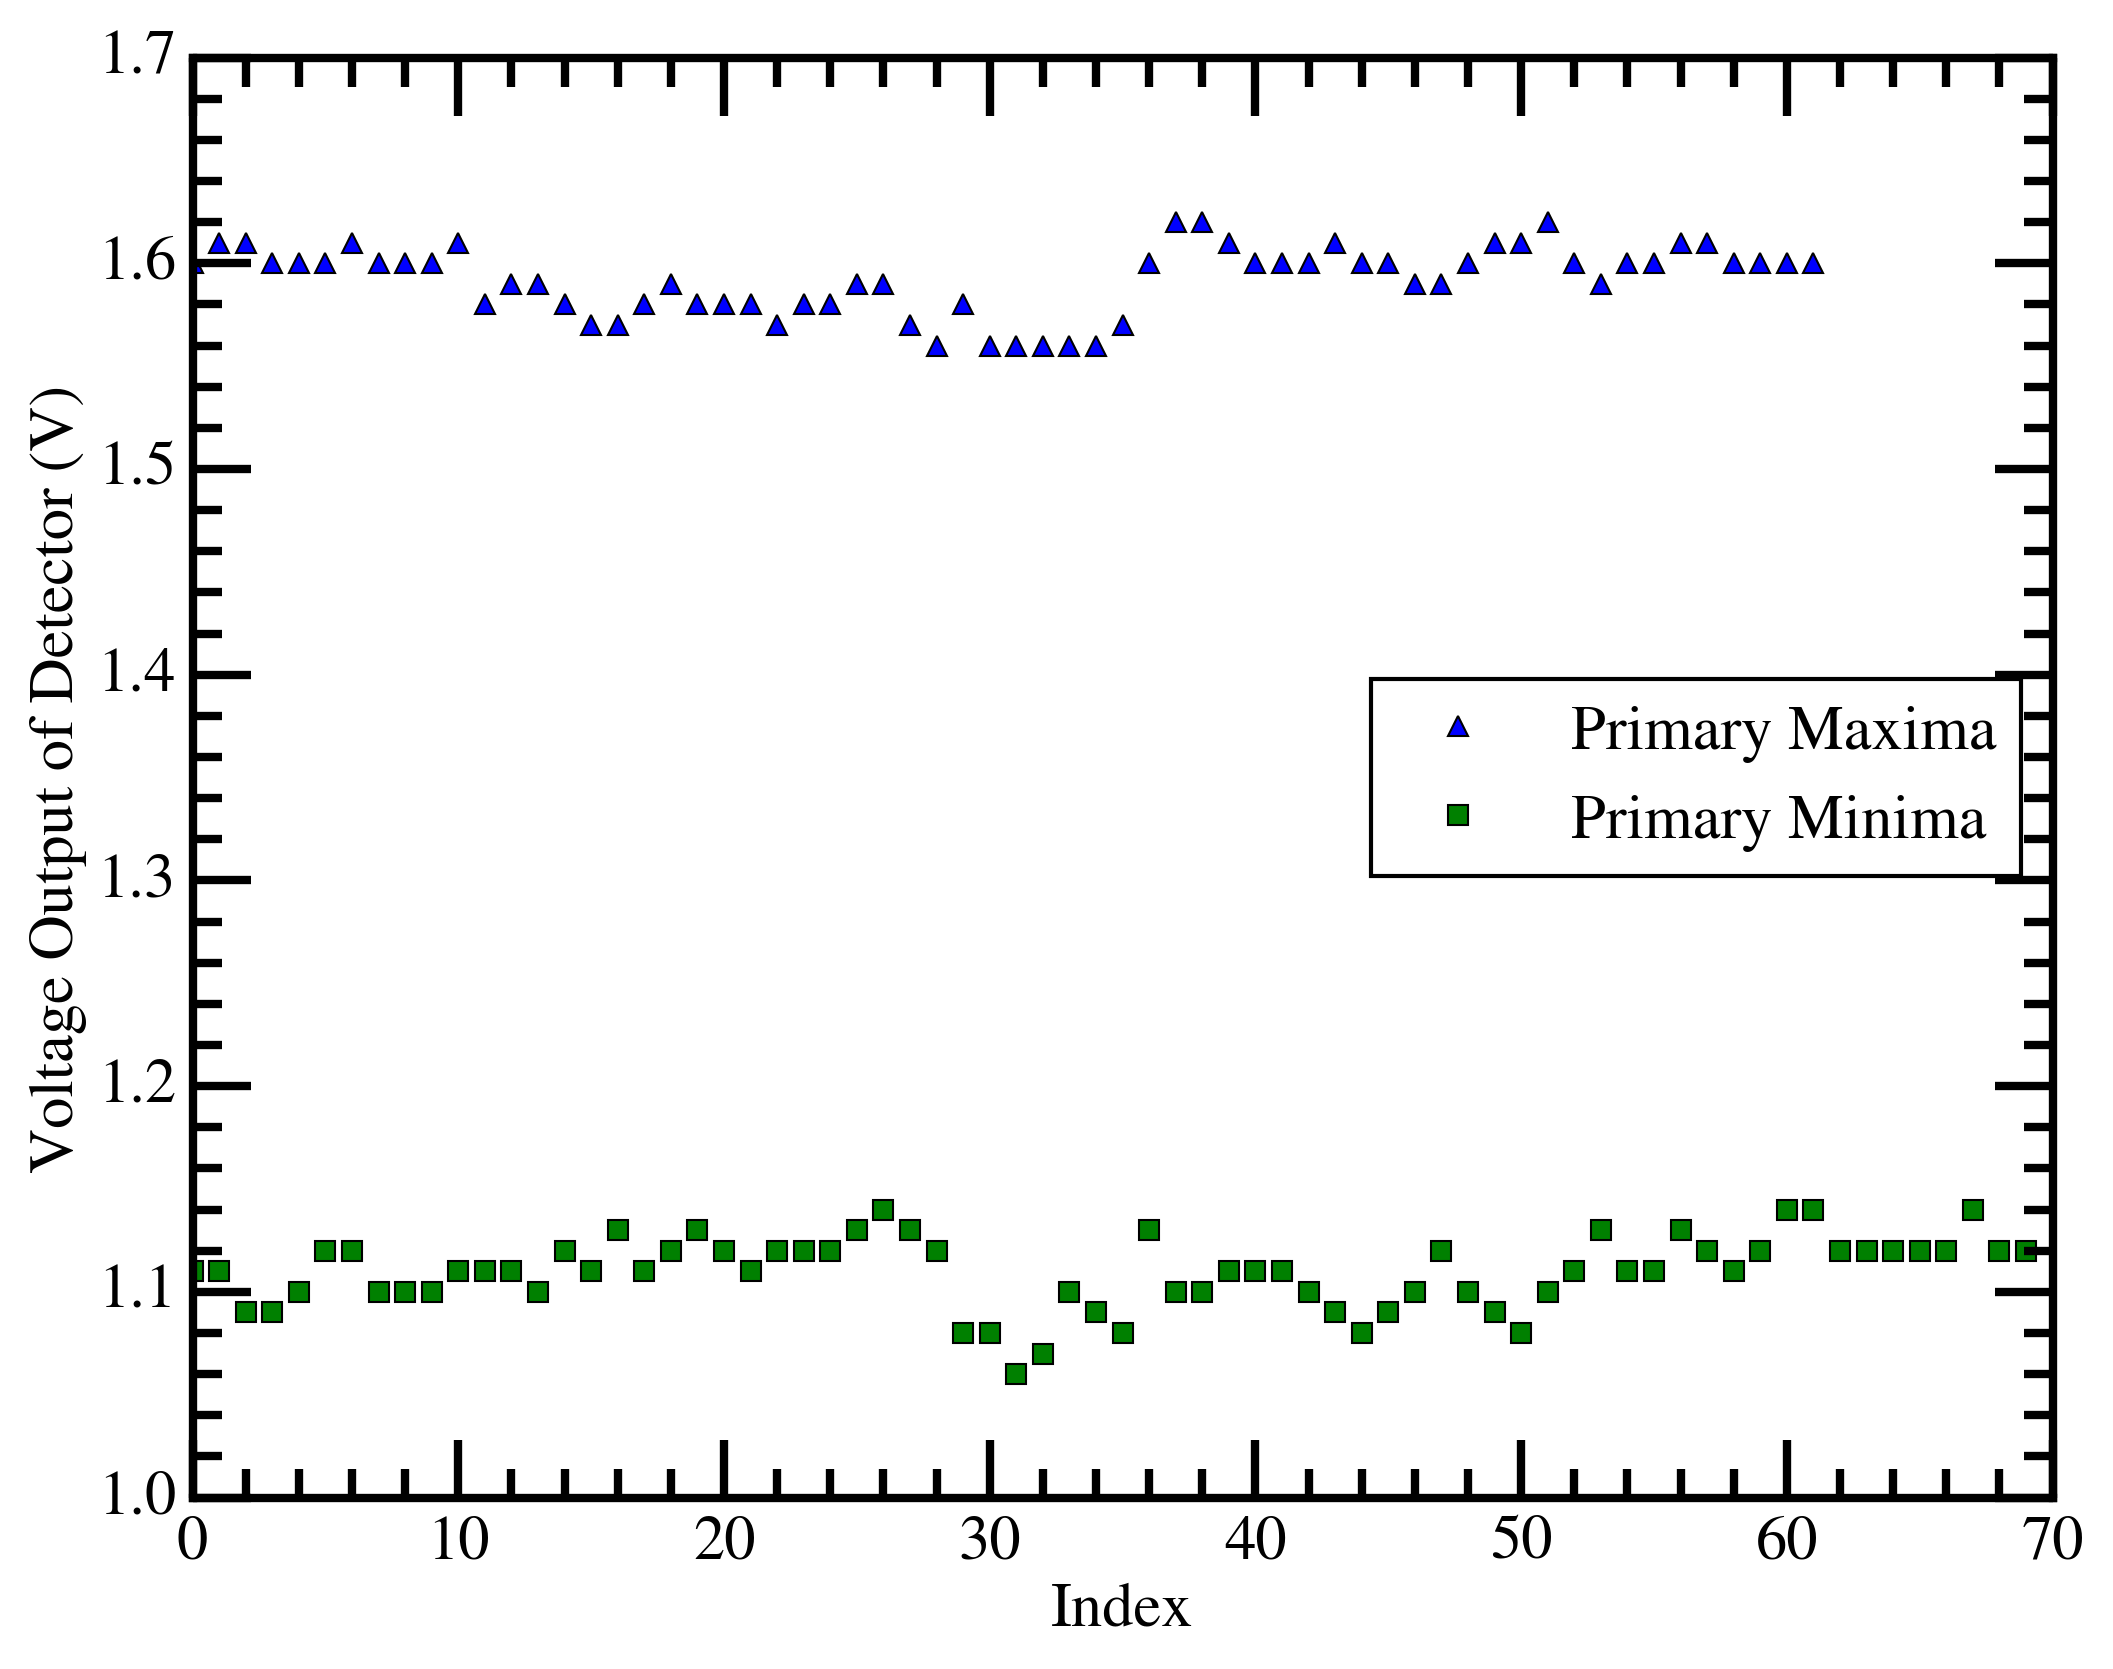
\includegraphics[width=0.8\textwidth]{fig/Intensity.png}
        \caption{Voltage output of photodiode corresponding to maxima and minima.}
    \end{figure}
\end{columns}

\end{frame}

\begin{frame}{Wavelength $601\pm37(\text{sys})\pm10(\text{stat})\text{nm}$ Matches the Color of the Laser}
\begin{columns}
    \column{0.5\textwidth}
    \begin{itemize}
        \item Measured voltage difference between peaks: $(3.192 \pm 0.055) \text{ V}$
        \item Calculated wavelength:
        \[
        \lambda = 601\pm37(\text{sys})\pm10(\text{stat})\text{ nm}
        \]
        \item Matches expected wavelength of the orange laser.
    \end{itemize}
    \column{0.5\textwidth}
        \begin{figure}
        \centering
        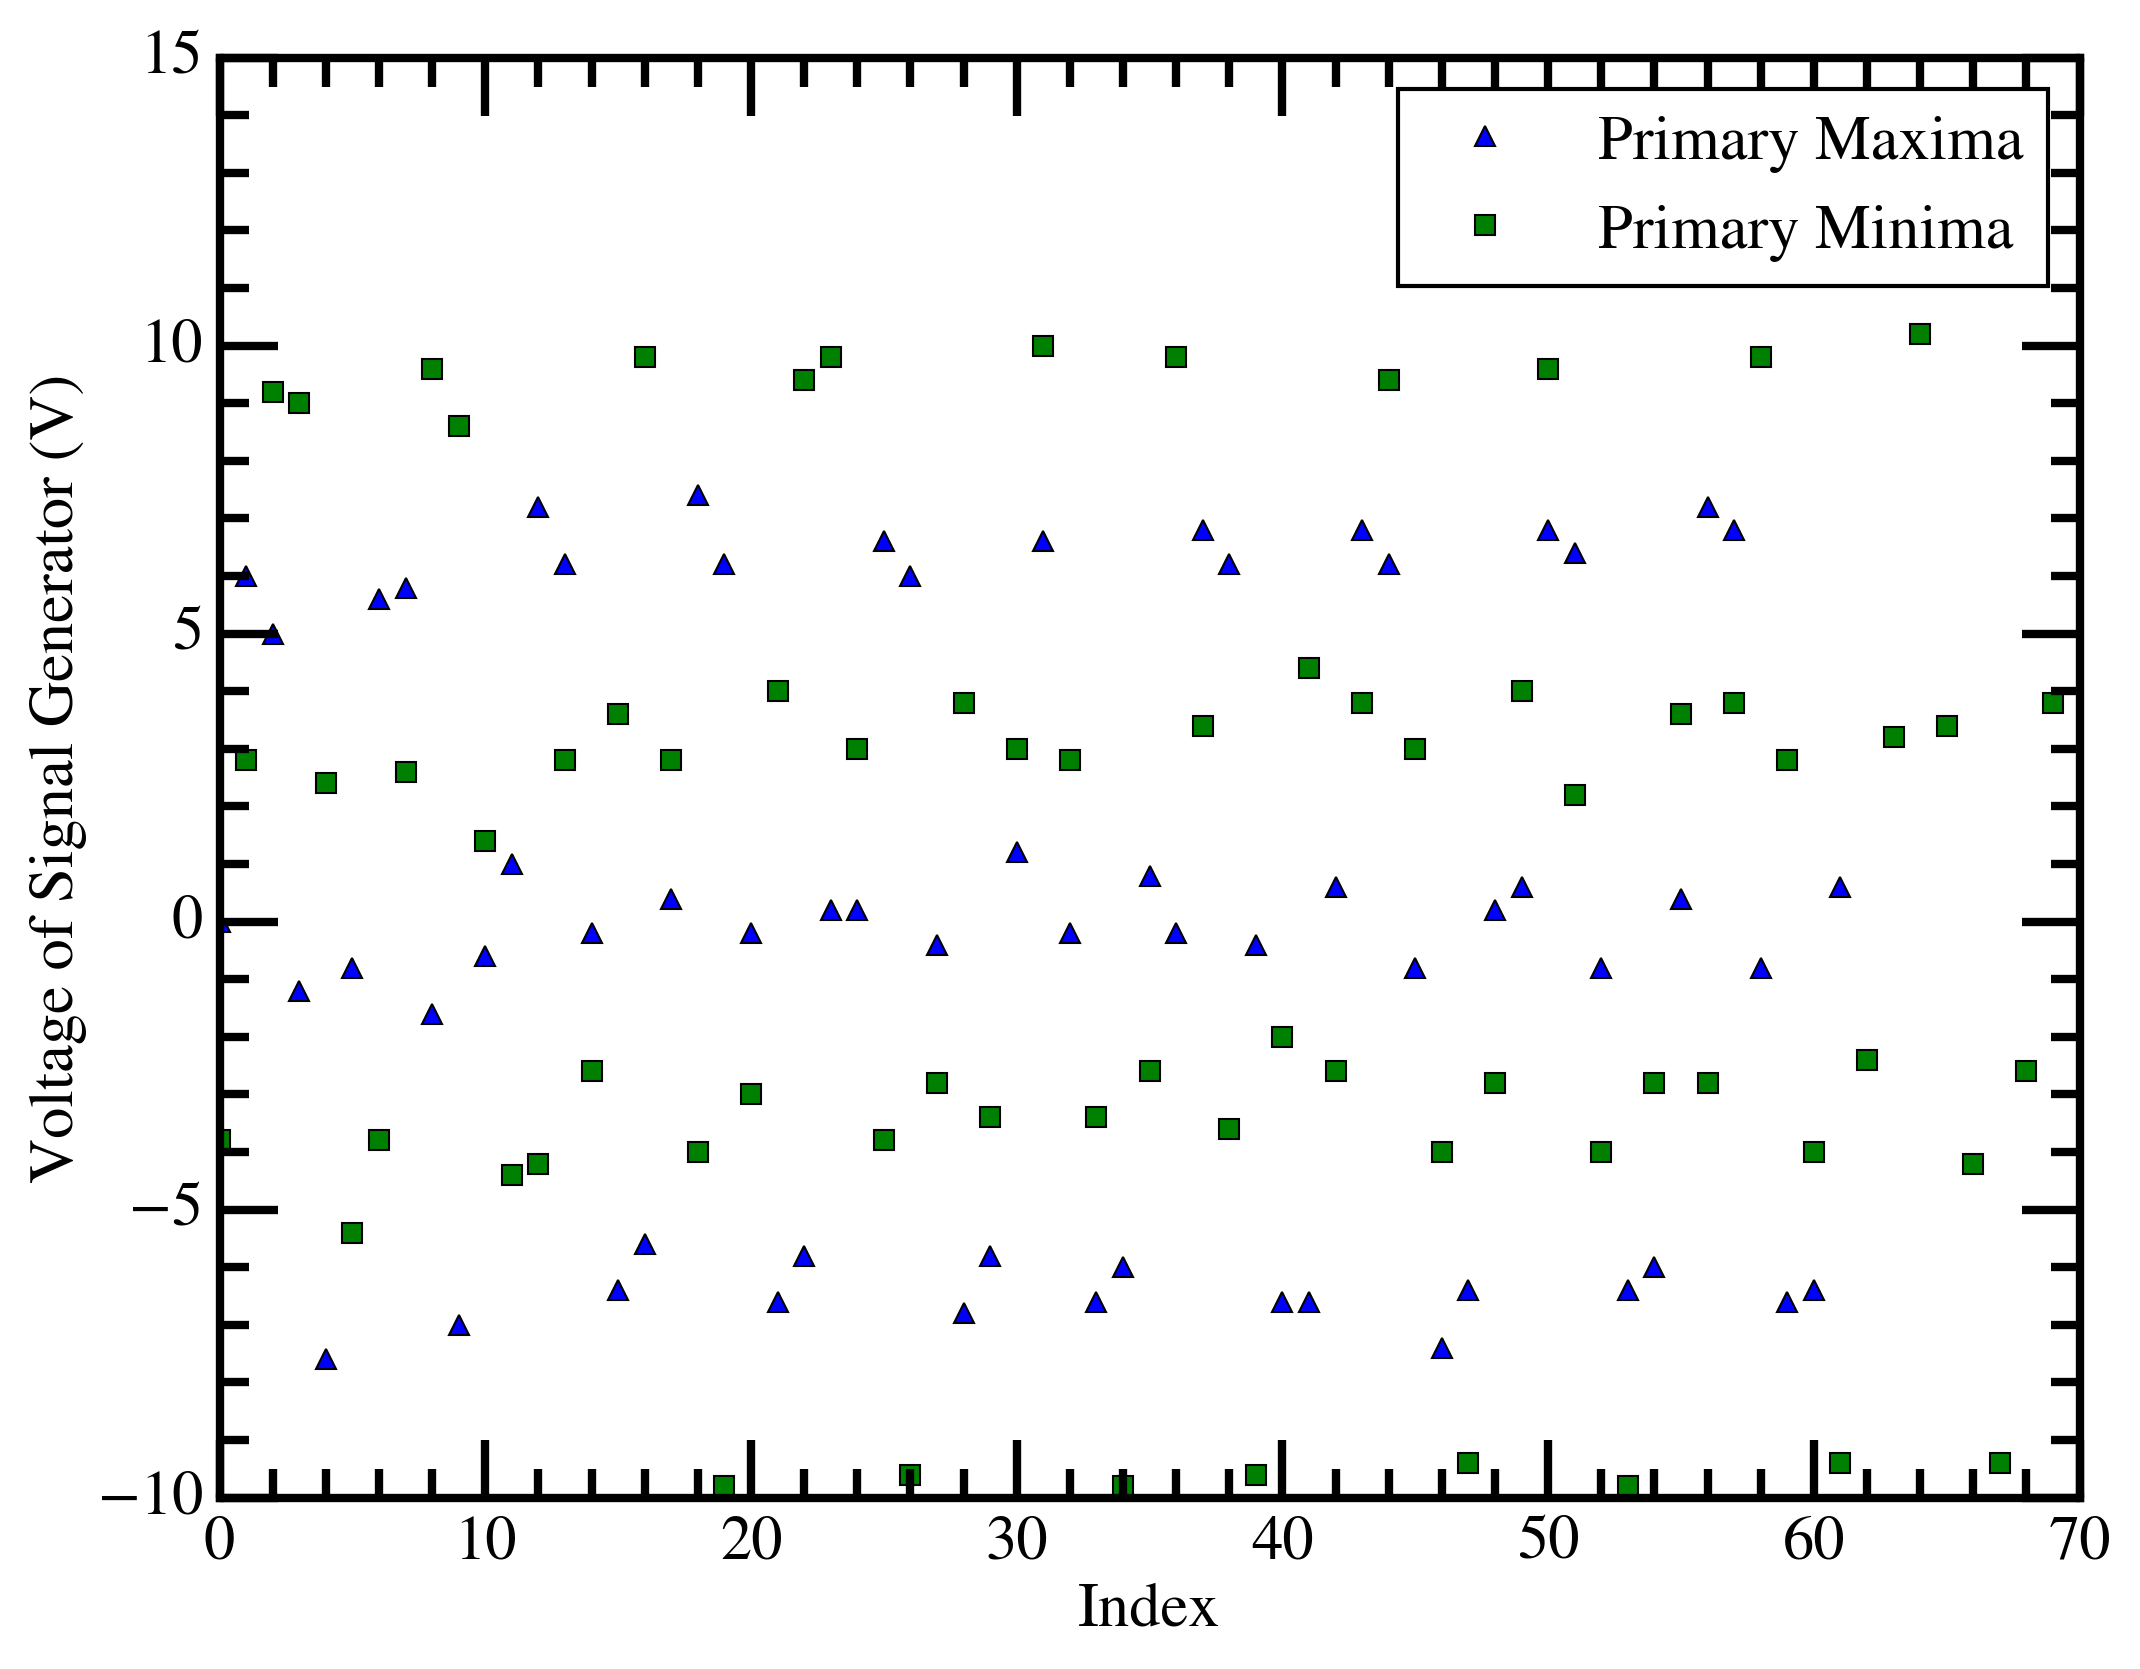
\includegraphics[width=0.8\textwidth]{fig/Primary_Maxima_Minima.png}
    \caption{Voltage at primary maxima and minima.}
    \end{figure}
\end{columns}
\end{frame}

% Uncertainty Analysis Slide
\begin{frame}{Uncertainty Dominated by Calibration of the Piezoelectric}
    \begin{itemize}
        \item \textbf{Systematic error}: Calibration of the piezoelectric device
        \[
        \delta \lambda = 37 \text{ nm}
        \]
        \item \textbf{Statistical error}: Peak detection noise
        \[
        \delta \lambda = 10 \text{ nm}
        \]
    \end{itemize}
\end{frame}

% Conclusion Slide
\section{Conclusion}
\begin{frame}{Conclusion and Future Improvements}
    \begin{itemize}
        \item Successfully measured the wavelength of an orange laser:
        \[
        601\pm37(\text{sys})\pm10(\text{stat})\text{ nm}
        \]
        \item Demonstrated interference and wave nature of light.
        \item Future improvements:
        \begin{itemize}
            \item Improve mirror alignment for higher visibility.
            \item Use a more precise piezoelectric transducer.
            \item Implement automated feedback to stabilize fringes.
        \end{itemize}
    \end{itemize}
\end{frame}

% Acknowledgments Slide
\begin{frame}{Acknowledgments}
Special thanks to J. Lewis, M. Bohdan, and V. Tran for assistance. Thanks to the MIT 8.13 teaching team for guidance. 
\end{frame}

% References Slide
\begin{frame}[allowframebreaks]{References}
    \bibliographystyle{unsrt}
    \bibliography{report_michelson_ref}
\end{frame}

\end{document}